% Options for packages loaded elsewhere
\PassOptionsToPackage{unicode}{hyperref}
\PassOptionsToPackage{hyphens}{url}
%
\documentclass[
]{book}
\usepackage{amsmath,amssymb}
\usepackage{iftex}
\ifPDFTeX
  \usepackage[T1]{fontenc}
  \usepackage[utf8]{inputenc}
  \usepackage{textcomp} % provide euro and other symbols
\else % if luatex or xetex
  \usepackage{unicode-math} % this also loads fontspec
  \defaultfontfeatures{Scale=MatchLowercase}
  \defaultfontfeatures[\rmfamily]{Ligatures=TeX,Scale=1}
\fi
\usepackage{lmodern}
\ifPDFTeX\else
  % xetex/luatex font selection
\fi
% Use upquote if available, for straight quotes in verbatim environments
\IfFileExists{upquote.sty}{\usepackage{upquote}}{}
\IfFileExists{microtype.sty}{% use microtype if available
  \usepackage[]{microtype}
  \UseMicrotypeSet[protrusion]{basicmath} % disable protrusion for tt fonts
}{}
\makeatletter
\@ifundefined{KOMAClassName}{% if non-KOMA class
  \IfFileExists{parskip.sty}{%
    \usepackage{parskip}
  }{% else
    \setlength{\parindent}{0pt}
    \setlength{\parskip}{6pt plus 2pt minus 1pt}}
}{% if KOMA class
  \KOMAoptions{parskip=half}}
\makeatother
\usepackage{xcolor}
\usepackage{color}
\usepackage{fancyvrb}
\newcommand{\VerbBar}{|}
\newcommand{\VERB}{\Verb[commandchars=\\\{\}]}
\DefineVerbatimEnvironment{Highlighting}{Verbatim}{commandchars=\\\{\}}
% Add ',fontsize=\small' for more characters per line
\usepackage{framed}
\definecolor{shadecolor}{RGB}{248,248,248}
\newenvironment{Shaded}{\begin{snugshade}}{\end{snugshade}}
\newcommand{\AlertTok}[1]{\textcolor[rgb]{0.94,0.16,0.16}{#1}}
\newcommand{\AnnotationTok}[1]{\textcolor[rgb]{0.56,0.35,0.01}{\textbf{\textit{#1}}}}
\newcommand{\AttributeTok}[1]{\textcolor[rgb]{0.13,0.29,0.53}{#1}}
\newcommand{\BaseNTok}[1]{\textcolor[rgb]{0.00,0.00,0.81}{#1}}
\newcommand{\BuiltInTok}[1]{#1}
\newcommand{\CharTok}[1]{\textcolor[rgb]{0.31,0.60,0.02}{#1}}
\newcommand{\CommentTok}[1]{\textcolor[rgb]{0.56,0.35,0.01}{\textit{#1}}}
\newcommand{\CommentVarTok}[1]{\textcolor[rgb]{0.56,0.35,0.01}{\textbf{\textit{#1}}}}
\newcommand{\ConstantTok}[1]{\textcolor[rgb]{0.56,0.35,0.01}{#1}}
\newcommand{\ControlFlowTok}[1]{\textcolor[rgb]{0.13,0.29,0.53}{\textbf{#1}}}
\newcommand{\DataTypeTok}[1]{\textcolor[rgb]{0.13,0.29,0.53}{#1}}
\newcommand{\DecValTok}[1]{\textcolor[rgb]{0.00,0.00,0.81}{#1}}
\newcommand{\DocumentationTok}[1]{\textcolor[rgb]{0.56,0.35,0.01}{\textbf{\textit{#1}}}}
\newcommand{\ErrorTok}[1]{\textcolor[rgb]{0.64,0.00,0.00}{\textbf{#1}}}
\newcommand{\ExtensionTok}[1]{#1}
\newcommand{\FloatTok}[1]{\textcolor[rgb]{0.00,0.00,0.81}{#1}}
\newcommand{\FunctionTok}[1]{\textcolor[rgb]{0.13,0.29,0.53}{\textbf{#1}}}
\newcommand{\ImportTok}[1]{#1}
\newcommand{\InformationTok}[1]{\textcolor[rgb]{0.56,0.35,0.01}{\textbf{\textit{#1}}}}
\newcommand{\KeywordTok}[1]{\textcolor[rgb]{0.13,0.29,0.53}{\textbf{#1}}}
\newcommand{\NormalTok}[1]{#1}
\newcommand{\OperatorTok}[1]{\textcolor[rgb]{0.81,0.36,0.00}{\textbf{#1}}}
\newcommand{\OtherTok}[1]{\textcolor[rgb]{0.56,0.35,0.01}{#1}}
\newcommand{\PreprocessorTok}[1]{\textcolor[rgb]{0.56,0.35,0.01}{\textit{#1}}}
\newcommand{\RegionMarkerTok}[1]{#1}
\newcommand{\SpecialCharTok}[1]{\textcolor[rgb]{0.81,0.36,0.00}{\textbf{#1}}}
\newcommand{\SpecialStringTok}[1]{\textcolor[rgb]{0.31,0.60,0.02}{#1}}
\newcommand{\StringTok}[1]{\textcolor[rgb]{0.31,0.60,0.02}{#1}}
\newcommand{\VariableTok}[1]{\textcolor[rgb]{0.00,0.00,0.00}{#1}}
\newcommand{\VerbatimStringTok}[1]{\textcolor[rgb]{0.31,0.60,0.02}{#1}}
\newcommand{\WarningTok}[1]{\textcolor[rgb]{0.56,0.35,0.01}{\textbf{\textit{#1}}}}
\usepackage{longtable,booktabs,array}
\usepackage{calc} % for calculating minipage widths
% Correct order of tables after \paragraph or \subparagraph
\usepackage{etoolbox}
\makeatletter
\patchcmd\longtable{\par}{\if@noskipsec\mbox{}\fi\par}{}{}
\makeatother
% Allow footnotes in longtable head/foot
\IfFileExists{footnotehyper.sty}{\usepackage{footnotehyper}}{\usepackage{footnote}}
\makesavenoteenv{longtable}
\usepackage{graphicx}
\makeatletter
\def\maxwidth{\ifdim\Gin@nat@width>\linewidth\linewidth\else\Gin@nat@width\fi}
\def\maxheight{\ifdim\Gin@nat@height>\textheight\textheight\else\Gin@nat@height\fi}
\makeatother
% Scale images if necessary, so that they will not overflow the page
% margins by default, and it is still possible to overwrite the defaults
% using explicit options in \includegraphics[width, height, ...]{}
\setkeys{Gin}{width=\maxwidth,height=\maxheight,keepaspectratio}
% Set default figure placement to htbp
\makeatletter
\def\fps@figure{htbp}
\makeatother
\setlength{\emergencystretch}{3em} % prevent overfull lines
\providecommand{\tightlist}{%
  \setlength{\itemsep}{0pt}\setlength{\parskip}{0pt}}
\setcounter{secnumdepth}{5}
\usepackage{booktabs}
\ifLuaTeX
  \usepackage{selnolig}  % disable illegal ligatures
\fi
\usepackage[]{natbib}
\bibliographystyle{plainnat}
\IfFileExists{bookmark.sty}{\usepackage{bookmark}}{\usepackage{hyperref}}
\IfFileExists{xurl.sty}{\usepackage{xurl}}{} % add URL line breaks if available
\urlstyle{same}
\hypersetup{
  pdftitle={R语言与生物统计(畜牧兽医篇)},
  pdfauthor={李任峰},
  hidelinks,
  pdfcreator={LaTeX via pandoc}}

\title{R语言与生物统计(畜牧兽医篇)}
\author{李任峰}
\date{2023-07-11}

\usepackage{amsthm}
\newtheorem{theorem}{Theorem}[chapter]
\newtheorem{lemma}{Lemma}[chapter]
\newtheorem{corollary}{Corollary}[chapter]
\newtheorem{proposition}{Proposition}[chapter]
\newtheorem{conjecture}{Conjecture}[chapter]
\theoremstyle{definition}
\newtheorem{definition}{Definition}[chapter]
\theoremstyle{definition}
\newtheorem{example}{Example}[chapter]
\theoremstyle{definition}
\newtheorem{exercise}{Exercise}[chapter]
\theoremstyle{definition}
\newtheorem{hypothesis}{Hypothesis}[chapter]
\theoremstyle{remark}
\newtheorem*{remark}{Remark}
\newtheorem*{solution}{Solution}
\begin{document}
\maketitle

{
\setcounter{tocdepth}{1}
\tableofcontents
}
\hypertarget{ux5e8fux8a00}{%
\chapter*{序言}\label{ux5e8fux8a00}}
\addcontentsline{toc}{chapter}{序言}

\hypertarget{footnotes-and-citations}{%
\chapter{Footnotes and citations}\label{footnotes-and-citations}}

\hypertarget{footnotes}{%
\section{Footnotes}\label{footnotes}}

Footnotes are put inside the square brackets after a caret \texttt{\^{}{[}{]}}. Like this one \footnote{This is a footnote.}.

\hypertarget{citations}{%
\section{Citations}\label{citations}}

Reference items in your bibliography file(s) using \texttt{@key}.

For example, we are using the \textbf{bookdown} package \citep{R-bookdown} (check out the last code chunk in index.Rmd to see how this citation key was added) in this sample book, which was built on top of R Markdown and \textbf{knitr} \citep{xie2015} (this citation was added manually in an external file book.bib).
Note that the \texttt{.bib} files need to be listed in the index.Rmd with the YAML \texttt{bibliography} key.

The RStudio Visual Markdown Editor can also make it easier to insert citations: \url{https://rstudio.github.io/visual-markdown-editing/\#/citations}

\hypertarget{ux7b2c1ux7ae0-rux8bedux8a00ux57faux7840}{%
\chapter*{第1章 R语言基础}\label{ux7b2c1ux7ae0-rux8bedux8a00ux57faux7840}}
\addcontentsline{toc}{chapter}{第1章 R语言基础}

All chapters start with a first-level heading followed by your chapter title, like the line above. There should be only one first-level heading (\texttt{\#}) per .Rmd file.

\hypertarget{ux8f6fux4ef6ux5b89ux88c5}{%
\section*{1.1 软件安装}\label{ux8f6fux4ef6ux5b89ux88c5}}
\addcontentsline{toc}{section}{1.1 软件安装}

All chapter sections start with a second-level (\texttt{\#\#}) or higher heading followed by your section title, like the sections above and below here. You can have as many as you want within a chapter.

\hypertarget{rux7684ux5b89ux88c5}{%
\subsection*{1.1.1 R的安装}\label{rux7684ux5b89ux88c5}}
\addcontentsline{toc}{subsection}{1.1.1 R的安装}

Chapters and sections are numbered by default. To un-number a heading, add a \texttt{\{.unnumbered\}} or the shorter \texttt{\{-\}} at the end of the heading, like in this section.

\begin{Shaded}
\begin{Highlighting}[]
\NormalTok{a}\OtherTok{\textless{}{-}} \FunctionTok{c}\NormalTok{(}\DecValTok{1}\NormalTok{,}\DecValTok{2}\NormalTok{,}\DecValTok{3}\NormalTok{)}
\NormalTok{b }\OtherTok{\textless{}{-}} \FunctionTok{c}\NormalTok{(}\DecValTok{8}\NormalTok{,}\DecValTok{9}\NormalTok{,}\DecValTok{10}\NormalTok{)}
\FunctionTok{plot}\NormalTok{(a,b)}
\end{Highlighting}
\end{Shaded}

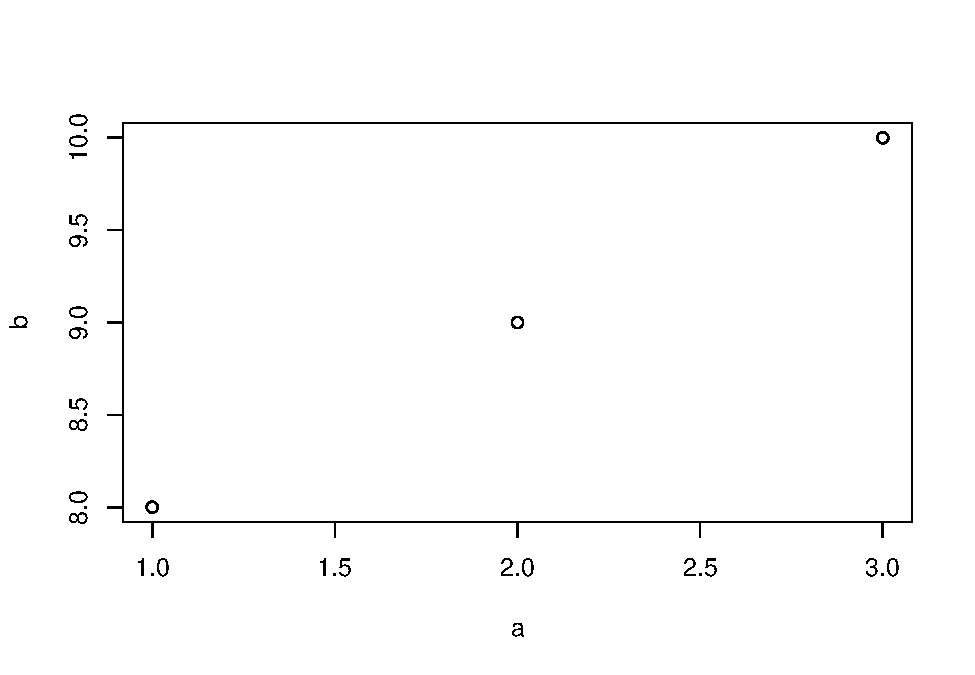
\includegraphics{_main_files/figure-latex/unnamed-chunk-1-1.pdf}

\hypertarget{rstudioux7684ux5b89ux88c5}{%
\subsection*{1.1.2 Rstudio的安装}\label{rstudioux7684ux5b89ux88c5}}
\addcontentsline{toc}{subsection}{1.1.2 Rstudio的安装}

\hypertarget{rux5305ux7684ux5b89ux88c5}{%
\subsection*{1.1.3 R包的安装}\label{rux5305ux7684ux5b89ux88c5}}
\addcontentsline{toc}{subsection}{1.1.3 R包的安装}

\hypertarget{ux6570ux636eux7c7bux578b}{%
\section*{1.2 数据类型}\label{ux6570ux636eux7c7bux578b}}
\addcontentsline{toc}{section}{1.2 数据类型}

\hypertarget{ux8f93ux5165ux6570ux636e}{%
\section*{1.3 输入数据}\label{ux8f93ux5165ux6570ux636e}}
\addcontentsline{toc}{section}{1.3 输入数据}

\hypertarget{ux7b2c2ux7ae0-ux6570ux636eux7ba1ux7406}{%
\chapter*{第2章 数据管理}\label{ux7b2c2ux7ae0-ux6570ux636eux7ba1ux7406}}
\addcontentsline{toc}{chapter}{第2章 数据管理}

Cross-references make it easier for your readers to find and link to elements in your book.

\hypertarget{ux7f3aux5931ux503cux5904ux7406}{%
\section*{2.1 缺失值处理}\label{ux7f3aux5931ux503cux5904ux7406}}
\addcontentsline{toc}{section}{2.1 缺失值处理}

There are two steps to cross-reference any heading:

\begin{enumerate}
\def\labelenumi{\arabic{enumi}.}
\tightlist
\item
  Label the heading: \texttt{\#\ Hello\ world\ \{\#nice-label\}}.

  \begin{itemize}
  \tightlist
  \item
    Leave the label off if you like the automated heading generated based on your heading title: for example, \texttt{\#\ Hello\ world} = \texttt{\#\ Hello\ world\ \{\#hello-world\}}.
  \item
    To label an un-numbered heading, use: \texttt{\#\ Hello\ world\ \{-\#nice-label\}} or \texttt{\{\#\ Hello\ world\ .unnumbered\}}.
  \end{itemize}
\item
  Next, reference the labeled heading anywhere in the text using \texttt{\textbackslash{}@ref(nice-label)}; for example, please see Chapter \ref{cross}.

  \begin{itemize}
  \tightlist
  \item
    If you prefer text as the link instead of a numbered reference use: \protect\hyperlink{cross}{any text you want can go here}.
  \end{itemize}
\end{enumerate}

\hypertarget{ux6570ux636eux7c7bux578bux8f6cux6362}{%
\section*{2.2 数据类型转换}\label{ux6570ux636eux7c7bux578bux8f6cux6362}}
\addcontentsline{toc}{section}{2.2 数据类型转换}

Figures and tables \emph{with captions} can also be cross-referenced from elsewhere in your book using \texttt{\textbackslash{}@ref(fig:chunk-label)} and \texttt{\textbackslash{}@ref(tab:chunk-label)}, respectively.

See Figure \ref{fig:nice-fig}.

\begin{Shaded}
\begin{Highlighting}[]
\FunctionTok{par}\NormalTok{(}\AttributeTok{mar =} \FunctionTok{c}\NormalTok{(}\DecValTok{4}\NormalTok{, }\DecValTok{4}\NormalTok{, .}\DecValTok{1}\NormalTok{, .}\DecValTok{1}\NormalTok{))}
\FunctionTok{plot}\NormalTok{(pressure, }\AttributeTok{type =} \StringTok{\textquotesingle{}b\textquotesingle{}}\NormalTok{, }\AttributeTok{pch =} \DecValTok{19}\NormalTok{)}
\end{Highlighting}
\end{Shaded}

\begin{figure}

{\centering 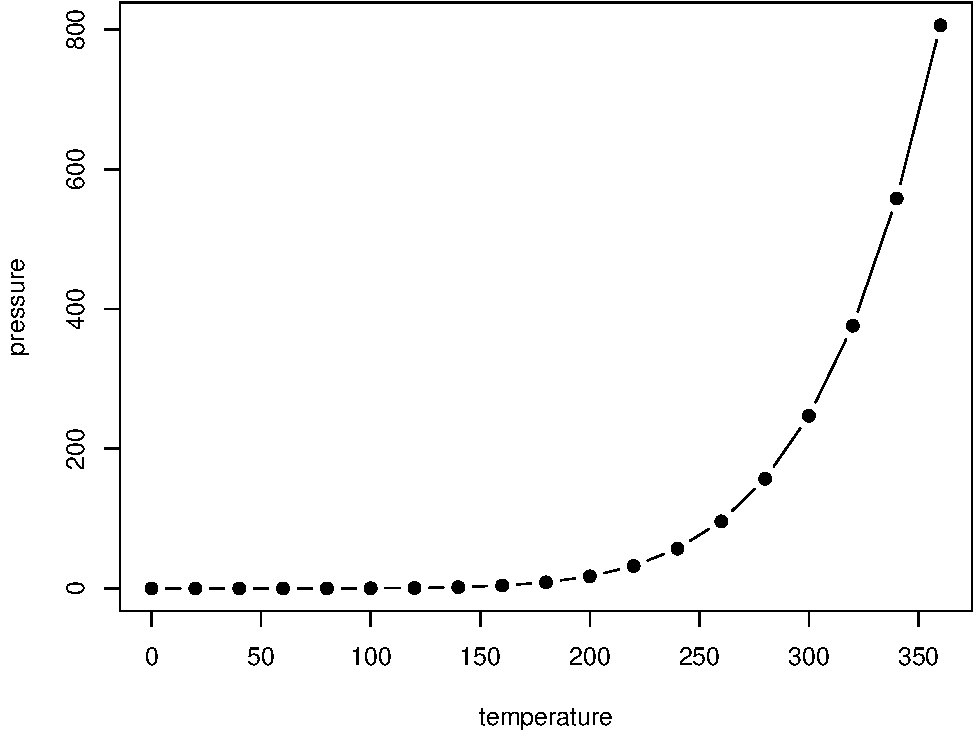
\includegraphics[width=0.8\linewidth]{_main_files/figure-latex/nice-fig-1} 

}

\caption{Here is a nice figure!}\label{fig:nice-fig}
\end{figure}

Don't miss Table \ref{tab:nice-tab}.

\begin{Shaded}
\begin{Highlighting}[]
\NormalTok{knitr}\SpecialCharTok{::}\FunctionTok{kable}\NormalTok{(}
  \FunctionTok{head}\NormalTok{(pressure, }\DecValTok{10}\NormalTok{), }\AttributeTok{caption =} \StringTok{\textquotesingle{}Here is a nice table!\textquotesingle{}}\NormalTok{,}
  \AttributeTok{booktabs =} \ConstantTok{TRUE}
\NormalTok{)}
\end{Highlighting}
\end{Shaded}

\begin{table}

\caption{\label{tab:nice-tab}Here is a nice table!}
\centering
\begin{tabular}[t]{rr}
\toprule
temperature & pressure\\
\midrule
0 & 0.0002\\
20 & 0.0012\\
40 & 0.0060\\
60 & 0.0300\\
80 & 0.0900\\
\addlinespace
100 & 0.2700\\
120 & 0.7500\\
140 & 1.8500\\
160 & 4.2000\\
180 & 8.8000\\
\bottomrule
\end{tabular}
\end{table}

\hypertarget{ux6570ux636eux6574ux7406}{%
\section*{2.3 数据整理}\label{ux6570ux636eux6574ux7406}}
\addcontentsline{toc}{section}{2.3 数据整理}

\hypertarget{ux7b2c3ux7ae0-rux4e0eux7edfux8ba1}{%
\chapter*{第3章 R与统计}\label{ux7b2c3ux7ae0-rux4e0eux7edfux8ba1}}
\addcontentsline{toc}{chapter}{第3章 R与统计}

You can add parts to organize one or more book chapters together. Parts can be inserted at the top of an .Rmd file, before the first-level chapter heading in that same file.

Add a numbered part: \texttt{\#\ (PART)\ Act\ one\ \{-\}} (followed by \texttt{\#\ A\ chapter})

Add an unnumbered part: \texttt{\#\ (PART\textbackslash{}*)\ Act\ one\ \{-\}} (followed by \texttt{\#\ A\ chapter})

Add an appendix as a special kind of un-numbered part: \texttt{\#\ (APPENDIX)\ Other\ stuff\ \{-\}} (followed by \texttt{\#\ A\ chapter}). Chapters in an appendix are prepended with letters instead of numbers.

\hypertarget{rux4e2dux7684ux57faux672cux7edfux8ba1ux51fdux6570}{%
\section*{3.1 R中的基本统计函数}\label{rux4e2dux7684ux57faux672cux7edfux8ba1ux51fdux6570}}
\addcontentsline{toc}{section}{3.1 R中的基本统计函数}

\begin{Shaded}
\begin{Highlighting}[]
\FunctionTok{load}\NormalTok{(}\StringTok{"C:/Users/liren/Desktop/R学习/在学/参考兽医统计教材/数据集/data\_rdata/data\_rdata/Data\_Set\_1.rdata"}\NormalTok{)}\CommentTok{\#加载数据}
\FunctionTok{head}\NormalTok{(data\_set\_1) }\CommentTok{\#查看数据前6行}
\end{Highlighting}
\end{Shaded}

\begin{verbatim}
##   Threshold
## 1       1.0
## 2       1.0
## 3       1.1
## 4       1.4
## 5       1.4
## 6       1.4
\end{verbatim}

\begin{Shaded}
\begin{Highlighting}[]
\FunctionTok{str}\NormalTok{(data\_set\_1) }\CommentTok{\#查看数据格式}
\end{Highlighting}
\end{Shaded}

\begin{verbatim}
## 'data.frame':    470 obs. of  1 variable:
##  $ Threshold: num  1 1 1.1 1.4 1.4 1.4 1.5 1.7 1.9 2 ...
##  - attr(*, "var.labels")= chr "Mechanical threshold (sheep)"
\end{verbatim}

\begin{Shaded}
\begin{Highlighting}[]
\FunctionTok{table}\NormalTok{(data\_set\_1) }\CommentTok{\#查看数据分布频率}
\end{Highlighting}
\end{Shaded}

\begin{verbatim}
## Threshold
##    1  1.1  1.4  1.5  1.7  1.9    2  2.1  2.2  2.3  2.4  2.5  2.6  2.7  2.8  2.9 
##    2    1    3    1    1    1    1    8    3    4    4    4    5    5    7    3 
##    3  3.1  3.2  3.3  3.4  3.5  3.6  3.7  3.8  3.9    4  4.1  4.2  4.3  4.4  4.5 
##    4   10   12    5    9   14   10    9   10    5    7   19   17   14    8   15 
##  4.6  4.7  4.8  4.9    5  5.1  5.2  5.3  5.4  5.5  5.6  5.7  5.8  5.9    6  6.1 
##   14   14   18   11    8    9    9    5    8    5    6    6    5    8    4    3 
##  6.2  6.3  6.4  6.5  6.6  6.7  6.8  6.9    7  7.1  7.2  7.4  7.5  7.6  7.7  7.8 
##    2    4    5    5    1    4    6    3    2    3    1    3    2    3    1    3 
##  7.9    8  8.1  8.2  8.3  8.4  8.5  8.6  8.7  8.8  8.9    9  9.1  9.2  9.3  9.4 
##    3    2    1    2    1    2    3    1    1    1    3    1    1    1    3    2 
##  9.5  9.6  9.7  9.8  9.9   10 10.2 10.3 10.4 10.5 10.7 10.8 10.9   11 11.3 11.5 
##    3    3    2    2    1    3    2    1    1    2    2    1    2    1    1    1 
## 11.8   12 12.3 12.4 12.6 12.8 12.9 13.4 13.8   14 14.5 14.9 
##    1    1    1    1    1    1    1    1    1    1    1    1
\end{verbatim}

\begin{Shaded}
\begin{Highlighting}[]
\FunctionTok{summary}\NormalTok{(data\_set\_1)}
\end{Highlighting}
\end{Shaded}

\begin{verbatim}
##    Threshold     
##  Min.   : 1.000  
##  1st Qu.: 3.700  
##  Median : 4.650  
##  Mean   : 5.252  
##  3rd Qu.: 6.100  
##  Max.   :14.900
\end{verbatim}

\hypertarget{ux57faux672cux7edfux8ba1ux51fdux6570}{%
\section*{3.2 基本统计函数}\label{ux57faux672cux7edfux8ba1ux51fdux6570}}
\addcontentsline{toc}{section}{3.2 基本统计函数}

\begin{Shaded}
\begin{Highlighting}[]
\FunctionTok{attach}\NormalTok{(data\_set\_1) }\CommentTok{\#当采用attach()时可不用$选取变量(注意:该方法容易造成变量操作混乱,一般不建议)。}
\FunctionTok{summary}\NormalTok{(data\_set\_1) }\CommentTok{\#summary()生成最大值、最小值、平均值、中位数、第1、3分位数等信息。另外,该函数可对矩阵、数据框、因子等多种类型的数据进行总结。}
\end{Highlighting}
\end{Shaded}

\begin{verbatim}
##    Threshold     
##  Min.   : 1.000  
##  1st Qu.: 3.700  
##  Median : 4.650  
##  Mean   : 5.252  
##  3rd Qu.: 6.100  
##  Max.   :14.900
\end{verbatim}

\begin{Shaded}
\begin{Highlighting}[]
\FunctionTok{table}\NormalTok{(data\_set\_1) }\CommentTok{\#用table()函数创建频率表,生成每个元素(或因子)出现的频数。}
\end{Highlighting}
\end{Shaded}

\begin{verbatim}
## Threshold
##    1  1.1  1.4  1.5  1.7  1.9    2  2.1  2.2  2.3  2.4  2.5  2.6  2.7  2.8  2.9 
##    2    1    3    1    1    1    1    8    3    4    4    4    5    5    7    3 
##    3  3.1  3.2  3.3  3.4  3.5  3.6  3.7  3.8  3.9    4  4.1  4.2  4.3  4.4  4.5 
##    4   10   12    5    9   14   10    9   10    5    7   19   17   14    8   15 
##  4.6  4.7  4.8  4.9    5  5.1  5.2  5.3  5.4  5.5  5.6  5.7  5.8  5.9    6  6.1 
##   14   14   18   11    8    9    9    5    8    5    6    6    5    8    4    3 
##  6.2  6.3  6.4  6.5  6.6  6.7  6.8  6.9    7  7.1  7.2  7.4  7.5  7.6  7.7  7.8 
##    2    4    5    5    1    4    6    3    2    3    1    3    2    3    1    3 
##  7.9    8  8.1  8.2  8.3  8.4  8.5  8.6  8.7  8.8  8.9    9  9.1  9.2  9.3  9.4 
##    3    2    1    2    1    2    3    1    1    1    3    1    1    1    3    2 
##  9.5  9.6  9.7  9.8  9.9   10 10.2 10.3 10.4 10.5 10.7 10.8 10.9   11 11.3 11.5 
##    3    3    2    2    1    3    2    1    1    2    2    1    2    1    1    1 
## 11.8   12 12.3 12.4 12.6 12.8 12.9 13.4 13.8   14 14.5 14.9 
##    1    1    1    1    1    1    1    1    1    1    1    1
\end{verbatim}

\begin{Shaded}
\begin{Highlighting}[]
\NormalTok{x }\OtherTok{\textless{}{-}} \FunctionTok{table}\NormalTok{(data\_set\_1)}
\FunctionTok{names}\NormalTok{(x)[}\FunctionTok{which}\NormalTok{(x}\SpecialCharTok{==}\FunctionTok{max}\NormalTok{(x))]}\CommentTok{\#查询出现频率最高的元素}
\end{Highlighting}
\end{Shaded}

\begin{verbatim}
## [1] "4.1"
\end{verbatim}

\begin{Shaded}
\begin{Highlighting}[]
\FunctionTok{min}\NormalTok{(data\_set\_1) }\CommentTok{\#查看最小值}
\end{Highlighting}
\end{Shaded}

\begin{verbatim}
## [1] 1
\end{verbatim}

\begin{Shaded}
\begin{Highlighting}[]
\FunctionTok{max}\NormalTok{(data\_set\_1) }\CommentTok{\#查看最大值}
\end{Highlighting}
\end{Shaded}

\begin{verbatim}
## [1] 14.9
\end{verbatim}

\begin{Shaded}
\begin{Highlighting}[]
\NormalTok{y }\OtherTok{\textless{}{-}} \FunctionTok{range}\NormalTok{(data\_set\_1) }\CommentTok{\#查看最大与最小值}
\FunctionTok{diff}\NormalTok{(y) }\CommentTok{\#查看最大与最小值之间的差值}
\end{Highlighting}
\end{Shaded}

\begin{verbatim}
## [1] 13.9
\end{verbatim}

\begin{Shaded}
\begin{Highlighting}[]
\FunctionTok{length}\NormalTok{(data\_set\_1)}
\end{Highlighting}
\end{Shaded}

\begin{verbatim}
## [1] 1
\end{verbatim}

\begin{Shaded}
\begin{Highlighting}[]
\FunctionTok{length}\NormalTok{(data\_set\_1}\SpecialCharTok{$}\NormalTok{Threshold) }\CommentTok{\#length()函数查看数据集中变量个数(数据容量)}
\end{Highlighting}
\end{Shaded}

\begin{verbatim}
## [1] 470
\end{verbatim}

\begin{Shaded}
\begin{Highlighting}[]
\FunctionTok{quantile}\NormalTok{(data\_set\_1}\SpecialCharTok{$}\NormalTok{Threshold)}
\end{Highlighting}
\end{Shaded}

\begin{verbatim}
##    0%   25%   50%   75%  100% 
##  1.00  3.70  4.65  6.10 14.90
\end{verbatim}

\begin{Shaded}
\begin{Highlighting}[]
\FunctionTok{quantile}\NormalTok{(data\_set\_1}\SpecialCharTok{$}\NormalTok{Threshold,}\FloatTok{0.25}\NormalTok{)}
\end{Highlighting}
\end{Shaded}

\begin{verbatim}
## 25% 
## 3.7
\end{verbatim}

\begin{Shaded}
\begin{Highlighting}[]
\FunctionTok{quantile}\NormalTok{(data\_set\_1}\SpecialCharTok{$}\NormalTok{Threshold,}\FloatTok{0.75}\NormalTok{)}
\end{Highlighting}
\end{Shaded}

\begin{verbatim}
## 75% 
## 6.1
\end{verbatim}

\begin{Shaded}
\begin{Highlighting}[]
\FunctionTok{IQR}\NormalTok{(data\_set\_1}\SpecialCharTok{$}\NormalTok{Threshold) }\CommentTok{\#计算四分位距(IQR),它是Q3和Q1之间的差值,即IQR = Q3 {-} Q1}
\end{Highlighting}
\end{Shaded}

\begin{verbatim}
## [1] 2.4
\end{verbatim}

\begin{Shaded}
\begin{Highlighting}[]
\FunctionTok{mean}\NormalTok{(Threshold) }\CommentTok{\#平均值(前面需先用attach()函数加载数据)}
\end{Highlighting}
\end{Shaded}

\begin{verbatim}
## [1] 5.251702
\end{verbatim}

\begin{Shaded}
\begin{Highlighting}[]
\FunctionTok{median}\NormalTok{(Threshold) }\CommentTok{\#中位数}
\end{Highlighting}
\end{Shaded}

\begin{verbatim}
## [1] 4.65
\end{verbatim}

\begin{Shaded}
\begin{Highlighting}[]
\FunctionTok{var}\NormalTok{(Threshold) }\CommentTok{\#求方差}
\end{Highlighting}
\end{Shaded}

\begin{verbatim}
## [1] 5.959731
\end{verbatim}

\begin{Shaded}
\begin{Highlighting}[]
\FunctionTok{sd}\NormalTok{(Threshold) }\CommentTok{\#求标准差}
\end{Highlighting}
\end{Shaded}

\begin{verbatim}
## [1] 2.441256
\end{verbatim}

\hypertarget{ux56deux5f52ux5206ux6790}{%
\section*{3.3 回归分析}\label{ux56deux5f52ux5206ux6790}}
\addcontentsline{toc}{section}{3.3 回归分析}

\hypertarget{ux7b2c4ux7ae0-rux8bedux8a00ux7ed8ux56fe}{%
\chapter*{第4章 R语言绘图}\label{ux7b2c4ux7ae0-rux8bedux8a00ux7ed8ux56fe}}
\addcontentsline{toc}{chapter}{第4章 R语言绘图}

\hypertarget{ux57faux672cux7ed8ux56fe}{%
\section*{4.1 基本绘图}\label{ux57faux672cux7ed8ux56fe}}
\addcontentsline{toc}{section}{4.1 基本绘图}

Footnotes are put inside the square brackets after a caret \texttt{\^{}{[}{]}}. Like this one \footnote{This is a footnote.}.

\hypertarget{ux9ad8ux7ea7ux7ed8ux56fe}{%
\section*{4.2 高级绘图}\label{ux9ad8ux7ea7ux7ed8ux56fe}}
\addcontentsline{toc}{section}{4.2 高级绘图}

Reference items in your bibliography file(s) using \texttt{@key}.

For example, we are using the \textbf{bookdown} package \citep{R-bookdown} (check out the last code chunk in index.Rmd to see how this citation key was added) in this sample book, which was built on top of R Markdown and \textbf{knitr} \citep{xie2015} (this citation was added manually in an external file book.bib).
Note that the \texttt{.bib} files need to be listed in the index.Rmd with the YAML \texttt{bibliography} key.

The RStudio Visual Markdown Editor can also make it easier to insert citations: \url{https://rstudio.github.io/visual-markdown-editing/\#/citations}

\hypertarget{ux7b2c5ux7ae0-rux8bedux8a00ux4e0eux673aux5668ux5b66ux4e60}{%
\chapter*{第5章 R语言与机器学习}\label{ux7b2c5ux7ae0-rux8bedux8a00ux4e0eux673aux5668ux5b66ux4e60}}
\addcontentsline{toc}{chapter}{第5章 R语言与机器学习}

\hypertarget{ux56deux5f52ux5206ux6790-1}{%
\section*{5.1 回归分析}\label{ux56deux5f52ux5206ux6790-1}}
\addcontentsline{toc}{section}{5.1 回归分析}

Here is an equation.

\begin{equation} 
  f\left(k\right) = \binom{n}{k} p^k\left(1-p\right)^{n-k}
  \label{eq:binom}
\end{equation}

You may refer to using \texttt{\textbackslash{}@ref(eq:binom)}, like see Equation \eqref{eq:binom}.

\hypertarget{ux805aux7c7bux5206ux6790}{%
\section*{5.2 聚类分析}\label{ux805aux7c7bux5206ux6790}}
\addcontentsline{toc}{section}{5.2 聚类分析}

Labeled theorems can be referenced in text using \texttt{\textbackslash{}@ref(thm:tri)}, for example, check out this smart theorem \ref{thm:tri}.

\begin{theorem}
\protect\hypertarget{thm:tri}{}\label{thm:tri}For a right triangle, if \(c\) denotes the \emph{length} of the hypotenuse
and \(a\) and \(b\) denote the lengths of the \textbf{other} two sides, we have
\[a^2 + b^2 = c^2\]
\end{theorem}

Read more here \url{https://bookdown.org/yihui/bookdown/markdown-extensions-by-bookdown.html}.

\hypertarget{ux8d1dux53f6ux65afux5206ux6790}{%
\section*{5.3 贝叶斯分析}\label{ux8d1dux53f6ux65afux5206ux6790}}
\addcontentsline{toc}{section}{5.3 贝叶斯分析}

The R Markdown Cookbook provides more help on how to use custom blocks to design your own callouts: \url{https://bookdown.org/yihui/rmarkdown-cookbook/custom-blocks.html}

\hypertarget{ux7b2c6ux7ae0-rux4e0eux667aux80fdux5316ux7f16ux7a0b}{%
\chapter*{第6章 R与智能化编程}\label{ux7b2c6ux7ae0-rux4e0eux667aux80fdux5316ux7f16ux7a0b}}
\addcontentsline{toc}{chapter}{第6章 R与智能化编程}

\hypertarget{publishing}{%
\section*{6.1 Publishing}\label{publishing}}
\addcontentsline{toc}{section}{6.1 Publishing}

HTML books can be published online, see: \url{https://bookdown.org/yihui/bookdown/publishing.html}

\hypertarget{pages}{%
\section*{6.2 404 pages}\label{pages}}
\addcontentsline{toc}{section}{6.2 404 pages}

By default, users will be directed to a 404 page if they try to access a webpage that cannot be found. If you'd like to customize your 404 page instead of using the default, you may add either a \texttt{\_404.Rmd} or \texttt{\_404.md} file to your project root and use code and/or Markdown syntax.

Bookdown HTML books will provide HTML metadata for social sharing on platforms like Twitter, Facebook, and LinkedIn, using information you provide in the \texttt{index.Rmd} YAML. To setup, set the \texttt{url} for your book and the path to your \texttt{cover-image} file. Your book's \texttt{title} and \texttt{description} are also used.

This \texttt{gitbook} uses the same social sharing data across all chapters in your book- all links shared will look the same.

Specify your book's source repository on GitHub using the \texttt{edit} key under the configuration options in the \texttt{\_output.yml} file, which allows users to suggest an edit by linking to a chapter's source file.

Read more about the features of this output format here:

\url{https://pkgs.rstudio.com/bookdown/reference/gitbook.html}

Or use:

\begin{Shaded}
\begin{Highlighting}[]
\NormalTok{?bookdown}\SpecialCharTok{::}\NormalTok{gitbook}
\end{Highlighting}
\end{Shaded}

\hypertarget{ux7b2c7ux7ae0-rux5728ux755cux7267ux517dux533bux9886ux57dfux7684ux5e94ux7528}{%
\chapter*{第7章 R在畜牧兽医领域的应用}\label{ux7b2c7ux7ae0-rux5728ux755cux7267ux517dux533bux9886ux57dfux7684ux5e94ux7528}}
\addcontentsline{toc}{chapter}{第7章 R在畜牧兽医领域的应用}

\hypertarget{publishing-1}{%
\section*{7.1 Publishing}\label{publishing-1}}
\addcontentsline{toc}{section}{7.1 Publishing}

HTML books can be published online, see: \url{https://bookdown.org/yihui/bookdown/publishing.html}

\hypertarget{pages-1}{%
\section*{7.2 404 pages}\label{pages-1}}
\addcontentsline{toc}{section}{7.2 404 pages}

By default, users will be directed to a 404 page if they try to access a webpage that cannot be found. If you'd like to customize your 404 page instead of using the default, you may add either a \texttt{\_404.Rmd} or \texttt{\_404.md} file to your project root and use code and/or Markdown syntax.

Bookdown HTML books will provide HTML metadata for social sharing on platforms like Twitter, Facebook, and LinkedIn, using information you provide in the \texttt{index.Rmd} YAML. To setup, set the \texttt{url} for your book and the path to your \texttt{cover-image} file. Your book's \texttt{title} and \texttt{description} are also used.

This \texttt{gitbook} uses the same social sharing data across all chapters in your book- all links shared will look the same.

Specify your book's source repository on GitHub using the \texttt{edit} key under the configuration options in the \texttt{\_output.yml} file, which allows users to suggest an edit by linking to a chapter's source file.

Read more about the features of this output format here:

\url{https://pkgs.rstudio.com/bookdown/reference/gitbook.html}

Or use:

\begin{Shaded}
\begin{Highlighting}[]
\NormalTok{?bookdown}\SpecialCharTok{::}\NormalTok{gitbook}
\end{Highlighting}
\end{Shaded}


  \bibliography{book.bib,packages.bib}

\end{document}
